      
               
                \begin{ledgroupsized}[r]{120mm}
                \footnotesize 
                \pstart                
                \selectlanguage{ngerman}
                \noindent\textbf{\"{U}berlieferung:}   
                \pend
                \end{ledgroupsized}
            
              
                            \begin{ledgroupsized}[r]{114mm}
                            \footnotesize 
                            \pstart \parindent -6mm
                            \makebox[6mm][l]{\textit{L}}Konzept: LH XXXV 5, 2 Bl. 5\textendash6. 1 Bog. 2\textsuperscript{o}. 4 S. Papier an den R\"{a}ndern zerbr\"{o}selt, z. T. eingerissen. Ecken teilweise abgebrochen, insbesondere fehlt ein gr\"{o}ßeres St\"{u}ck der rechten unteren Ecke von Bl. 6 r\textsuperscript{o}. Dadurch Textverluste. Kleinere L\"{o}cher im unteren Teil von Bl. 5. Auf allen Seiten Zeichnungen bzw. Grafiken, die in den Text integriert sind. Textfolge: Bl. 6 r\textsuperscript{o}, Bl. 6 v\textsuperscript{o}, Bl. 5 r\textsuperscript{o} [\textit{Teil~1}], Bl. 5 v\textsuperscript{o} [\textit{Teil 2}]. Die Wiedergabe des Textes als einheitliches, jedoch aus zwei Teilen bestehendes St\"{u}ck, st\"{u}tzt sich auf die folgende Randbemerkung von Bl. 5 v\textsuperscript{o}: Demonstratio accurata quae vero tribus paginis praecedentibus continentur lapsibus plena sunt quorum origines ibi in margine notavi. Die Ergebnisse von Bl. 5 v\textsuperscript{o} werden zum Ausgangspunkt f\"{u}r eine nochmalige Durchsicht der vor\-ausgehenden Textteile und f\"{u}hren zu umfangreichen Streichungen. Die Gr\"{u}nde f\"{u}r die Streichungen sowie f\"{u}r das Beibehalten der einzelnen Textpassagen werden von Leibniz in kurzen Kommentaren erl\"{a}utert. Die in Kleindruck gesetzten Teile von Bl. 6 r\textsuperscript{o} und Bl. 6 v\textsuperscript{o} sind in der Handschrift gestrichen. Datierung, Titel und Hinweis auf \cite{00261}\textit{LSB} VII, 3 N. 39 sowie LH XXXV 5, 2 Bl. 1 wurden sp\"{a}ter hinzugef\"{u}gt. \\Cc 2, Nr. 822 
                            \pend
                             \end{ledgroupsized}
                     
                %\normalsize
                \vspace*{5mm}
                \begin{ledgroup}
                \footnotesize 
                \pstart
            \noindent\footnotesize{\textbf{Datierungsgr\"{u}nde}: Von Leibniz auf Bl. 6 r\textsuperscript{o} datiert.}
                \pend
                \end{ledgroup}
            
                \vspace*{8mm}
                \pstart 
                \normalsize\selectlanguage{latin}
            [6 r\textsuperscript{o}] Xb 1674.\footnote{\textit{Am oberen Rand rechts}: Adde schediasma de progressionibus et Geometria arcana et methodo Tangentium, item schediasma de Methodo Tangentium inversa exemplum, eod$\langle$em mense.$\rangle$}
            \pend 
               \pstart \begin{center}{\textso{Schediasma de Calculo Elastico}}\\\rule[0cm]{0cm}{0.7cm} 
               \lbrack\textit{Teil 1}\rbrack\end{center} 
                  \edtext{}{\lemma{mense.$\rangle$}\linenum{|25|||25|}\Bfootnote{Vgl. \cite{00261}\textit{LSB} VII, 3 N. 39 sowie LH XXXV 5, 2 Bl. 1}}
\pend
               \pstart\footnotesize Cum viderem \edtext{accelerationem\protect\index{Sachverzeichnis}{acceleratio} gravium cadentium}{\lemma{viderem}\Afootnote{ \textit{ (1) }\ staticen \textit{ (2) }\ cadentium \textit{ (3) }\ accelerationem gravium cadentium \textit{ L}}}
             praeclaris summorum Geometrarum Galilaei\protect\index{Namensregister}{\textso{Galilei} (Galilaeus, Galileus), Galileo 1564\textendash 1642} et Hugenii\protect\index{Namensregister}{\textso{Huygens} (Hugenius, Vgenius, Hugens, Huguens), Christiaan 1629\textendash 1695} inventis \edtext{ad certas quasdam leges revocatam}{\lemma{inventis}\Afootnote{ \textit{ (1) }\ sub leg \textit{ (2) }\ certis legibus subjectam \textit{ (3) }\ ad certas quasdam leges revocatam \textit{ L}}}; ad Elateria\protect\index{Sachverzeichnis}{elaterium} gradum putavi promovendum, intacta fere Geometris, et certe non paulo intractabiliora. Eligam autem in exemplum considerationem Elaterii\protect\index{Sachverzeichnis}{elaterium} simplicissimi et purissimi, scilicet quod in aere \edtext{deprehensum est}{\lemma{aere}\Afootnote{ \textit{ (1) }\ extra controversiam \textit{ (2) }\ deprehensum est \textit{ L}}}.
         Sit massa aeris\protect\index{Sachverzeichnis}{massa!aeris} capax replendi \edtext{naturaliter}{\lemma{}\Afootnote{naturaliter \textit{ erg.} \textit{ L}}} rectanguli solidi \textit{ABCD} redacta intra spatium \textit{BEFC}. In producta \textit{BC} sumatur recta \textit{CG}, jungaturque \textit{DG} et ipsi \textit{CG} parallela ducatur \textit{FH}.\pend 
%    Zeitz auskommentiert                      \begin{center}                   
%                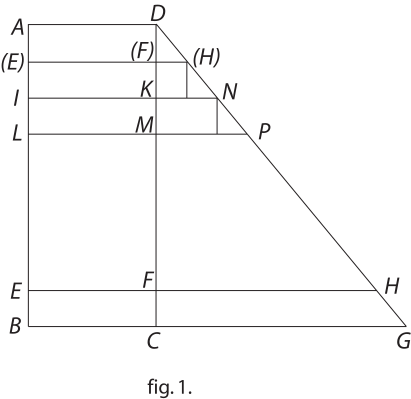
\includegraphics[width=0.5\textwidth]{images/35_5_6r1}
%                        %\caption{Bildbeschreibung}
%                        \end{center}
                     \pstart \footnotesize Cum omnis vis quam aer ad se restituendum exercet, oriatur a parvitate spatii materiam continente, manifestum est, aequalibus spatii decrementis aequalia esse virium incrementa\protect\index{Sachverzeichnis}{incrementum!virium}.\footnote{\textit{Links neben dem Text auf H\"{o}he der mit} aequalia esse \textit{beginnenden Zeile}: \textso{Error}} 
\pend 
\pstart 
\footnotesize Ductis ergo rectis Basi \textit{BC} parallelis numero infinitis, \textit{AD}, \textit{(E)(H)}, \textit{IK}, \textit{LM} aequalibus intervallis \edtext{\textit{AE}, \textit{EI}, \textit{IL}, distantibus}{\lemma{intervallis}\Afootnote{ \textit{ (1) }\ \textit{EI} distantibus \textit{ (2) }\ \textit{AE}, \textit{EI}, \textit{IL}, distantibus \textit{ L}}}. Patet operculo quodam \edtext{rigido}{\lemma{quodam}\Afootnote{ \textit{ (1) }\ solido \textit{ (2) }\ rigido \textit{ L}}} \textit{AD} uniformiter versus \textit{BC} progrediente \edtext{percurri}{\lemma{progrediente}\Afootnote{ \textit{ (1) }\ aequalibus temporibus aequalia \textit{ (2) }\ percurri \textit{ L}}} \edtext{sive aeri ab operculo adimi}{\lemma{sive}\Afootnote{aeri ab operculo adimi \textit{ erg.} \textit{ L}}} spatia \textit{AEFD}, \textit{EIKF}, \textit{ILMK} etc. \edtext{inter se aequalia}{\lemma{}\Afootnote{inter se aequalia \textit{ erg.} \textit{ L}}} adeoque aequalia esse virium Elaterii\protect\index{Sachverzeichnis}{elaterium} incrementa\protect\index{Sachverzeichnis}{incrementum!virium}. \edtext{Unde}{\lemma{incrementa.}\Afootnote{ \textit{ (1) }\ Quod si ergo \textit{ (2) }\ Unde \textit{ L}}} sequitur \edtext{vires}{\lemma{sequitur}\Afootnote{ \textit{ (1) }\ virium progressione \textit{ (2) }\ vires \textit{ L}}} Elaterii\protect\index{Sachverzeichnis}{elaterium} \edtext{quovis loco}{\lemma{quovis}\Afootnote{ \textit{ (1) }\ tempore \textit{ (2) }\ loco \textit{ L}}} quaesitas, repraesentari posse \edtext{Trianguli \textit{DCG} applicatis}{\lemma{posse}\Afootnote{ \textit{ (1) }\ applicatis \textit{ (2) }\ Trianguli   \textbar\ \textit{DCG} applicatis \textit{ erg.}\ \textbar\  \textit{ L}}}, \textit{(F)(H)}, \textit{KN}, \textit{MP} cum applicatas Trianguli uniformiter crescere constet. Vis ergo quaesita \edtext{operculo existente in \textit{IK}, est ad vim}{\lemma{quaesita}\Afootnote{ \textit{ (1) }\ in \textit{L}, erit ad vim \textit{ (2) }\ operculo [...] vim \textit{ L}}} quaesitam operculo existente in \textit{LM} ut Triangulum \textit{DKN}, ad Triangulum \textit{DMP}. 
\pend 
\pstart  
\footnotesize Eadem valet demonstratio si \textit{ABCD} sit \edtext{cylinder}{\lemma{sit}\Afootnote{ \textit{ (1) }\ columnare \textit{ (2) }\ cylinder \textit{ L}}}, aut prisma vel cylindricum quodlibet. Sed si sit conoeides parabolicum, et loco trianguli \textit{DCG} describenda erit parabola; si sit conus vel sphaera \edtext{describendae erunt parabolae cubicae}{\lemma{sphaera}\Afootnote{ \textit{ (1) }\ describenda erit parabola cubica \textit{ (2) }\ describendae erunt parabolae cubicae \textit{ L}}}\edtext{}{\lemma{}\Afootnote{cubicae  \textbar\ sed modo convexa modo concava \textit{ erg. u.}\  \textit{ gestr.}\ \textbar\ quae \textit{ L}}} quae satis paradoxa \edtext{videbuntur}{\lemma{}\Afootnote{videbuntur \textit{ erg.} \textit{ L}}} rationem non intelligenti. Cum autem Elateria\protect\index{Sachverzeichnis}{elaterium} quibus in Automatis\protect\index{Sachverzeichnis}{automatum} utimur in spiram\protect\index{Sachverzeichnis}{spira} intorta esse soleant; eam utique formam considerare operae pretium erit, ut \edtext{discamus}{\lemma{ut}\Afootnote{ \textit{ (1) }\ certis \textit{ (2) }\ discamus \textit{ L}}} qua ratione fusi ad aequabilitatem motus considerandam additi, deminutio, Geometrica lege fieri debeat: quam artifices postea quantum licet in materia exprimere possint. \edtext{Sed de eo quidem postea, nunc non vires tantum}{\lemma{possint.}\Afootnote{ \textit{ (1) }\ Sed cum ille sit potiss \textit{ (2) }\ Sed [...] tantum \textit{ L}}} sed et accelerationes\protect\index{Sachverzeichnis}{acceleratio} Elaterii\protect\index{Sachverzeichnis}{elaterium} inter restituendum consideremus. Manifestum est autem ex his quae diximus, ut sunt in descensu gravium celeritates\protect\index{Sachverzeichnis}{celeritas} seu vires pro ratione temporum, ita esse in Elaterio\protect\index{Sachverzeichnis}{elaterium} cylindrico vires seu resistentias pro ratione locorum. 
\pend 
\pstart \footnotesize Sed ut de temporibus quoque ratiocinemur, ponamus operculum \textit{AD} operari pondere, quod aequale sit Elaterio aeris\protect\index{Sachverzeichnis}{elaterium!aeris} compressi in \textit{EF} ac proinde ei eousque comprimendo par futurum. Patet hujus ponderis\protect\index{Sachverzeichnis}{pondus} vim progressu continue \edtext{decrescere, quod resistentiam}{\lemma{decrescere,}\Afootnote{ \textit{ (1) }\ ob resi \textit{ (2) }\ quod resistentiam \textit{ L}}} semper majorem inveniat. Itaque initio in \textit{A} ejus vis erit ut \textit{DFH}, \edtext{at}{\lemma{\textit{DFH,}}\Afootnote{ \textit{ (1) }\ in \textit{(E)} erit \textit{ (2) }\ at \textit{ L}}} in \textit{I} erit \textit{KNHF}, in \textit{L} erit \textit{MPHF}, donec in \textit{E} plane destruatur et evanescat. \edtext{Et}{\lemma{evanescat.}\Afootnote{ \textit{ (1) }\ Sed \textit{ (2) }\ Et \textit{ L}}} haec quidem ita habent si nulla aut detrimento\protect\index{Sachverzeichnis}{detrimentum} parietis vasis destructa esse intelligatur ponderis\protect\index{Sachverzeichnis}{pondus} inter descendendum quaesita acceleratio\protect\index{Sachverzeichnis}{acceleratio}. 
            \pend               
%  Zeitz auskommentiert                    \begin{center}                    
%                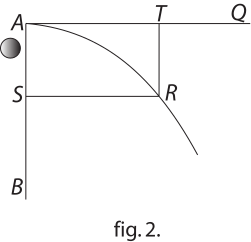
\includegraphics[width=0.3\textwidth]{images/35_5_6r2}
%                        %\caption{Bildbeschreibung}
%                        \end{center}
                        \pstart \footnotesize Sed si illam quoque in rationes venire velimus paulo subtilior sese inquisitio offert. Primum si pondus\protect\index{Sachverzeichnis}{pondus} quoddam per perpendicularem tempore \textit{AQ} descendat motu gravitatis constat ex demonstratis a Galilaeo\protect\index{Namensregister}{\textso{Galilei} (Galilaeus, Galileus), Galileo 1564\textendash 1642} spatia 
                        %@ @ @ Dies ist eine Abstandszeile - fuer den Fall, dass mehrere figures hintereinander kommen, ohne dass dazwischen laengerer Text steht. Dies kann zu einer Fahlermeldung fuehren. @ @ @ \\
                     fig. 2. percursa fore in duplicata temporum ratione descripta ergo parabola \textit{AR}, cujus axis \textit{AB} tangens verticis \textit{ATQ}. Si tempora sint ut \textit{AT}, spatia fore ut \textit{TR} applicatae ad tangentem verticis. Quod si contra spatia sint ut  \edtext{\textit{AS} abscissae}{\lemma{\textit{AS}}\Afootnote{ \textit{ (1) }\ partes \textit{A} \textit{ (2) }\ abscissae \textit{ L}\hspace{10cm}}} ex axe, erunt tempora ut \textit{SR} ordinatae parabolae ad axem.
\pend  
%   Zeitz auskommentiert                   \begin{center}                    
%                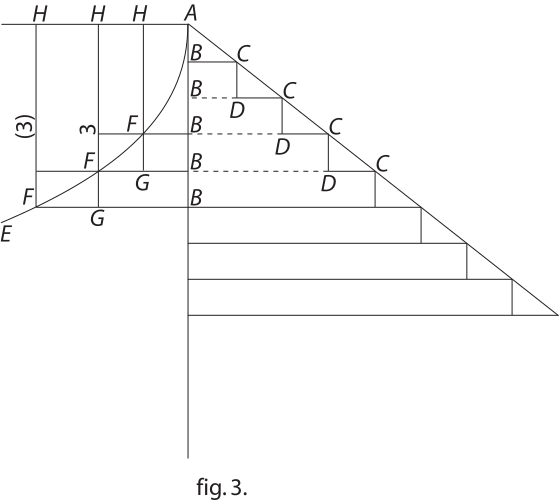
\includegraphics[width=0.55\textwidth]{images/35_5_6r3}
%                        %\caption{Bildbeschreibung}
%                        \end{center}
                        %@ @ @ Dies ist eine Abstandszeile - fuer den Fall, dass mehrere figures hintereinander kommen, ohne dass dazwischen laengerer Text steht. Dies kann zu einer Fahlermeldung fuehren. @ @ @ \\
                     \pstart 
                     Si\footnote{\textit{Quer zum Text. Bezugstext}: Si tempora sunt [...] spatiorum ratione, \textit{durch geschweifte Klammer markiert}: Demonstratio verissima satis elegans.} tempora sint \textit{AB} \edtext{fig. 3.}{\lemma{fig. 3.}\Afootnote{\textit{erg.} \textit{ L}}} celeritates\protect\index{Sachverzeichnis}{celeritas} quaesitae\footnote{\textit{Randbemerkung zu} celeritates quaesitae: non incrementa} \textit{CD} \edtext{erunt celeritates}{\lemma{erunt}\Afootnote{ \textit{ (1) }\ vires \textit{ (2) }\ celeritates \textit{ L}}} quaesitae \textit{BC}. \edtext{Sit}{\lemma{\textit{BC.}}\Afootnote{ \textit{ (1) }\ Spatia autem qu \textit{ (2) }\ Sit \textit{ L}}} \textit{AFE} parabola cujus vertex \textit{A} Tangens verticis \textit{AB} \edtext{et tangenti}{\lemma{}\Afootnote{et tangenti \textit{ erg.} \textit{ L}}} applicatae \textit{BF} et \textit{FG} ipsis \textit{AB} vel \textit{BC} \edtext{proportionales. Patet}{\lemma{proportionales.}\Afootnote{ \textit{ (1) }\ Ergo abscissae ex axe \textit{AH} $\sqcap$ \textit{BF}. \textit{ (2) }\ Patet \textit{ L}}} cum \textit{AB} sint tempora \edtext{incrementa uniformia \textit{DC} celeritates}{\lemma{tempora}\Afootnote{ \textit{ (1) }\ vires \textit{ (2) }\ incrementa  \textit{(a)}\ virium\protect\index{Sachverzeichnis}{incrementum!virium|textit} \textit{(b)}\ uniformia \textit{DC}  \textit{(aa)}\ vires \textit{(bb)}\ celeritates \textit{ L}}} quolibet momento \textit{B} quaesitae \textit{BC}, spatia infinite parva quolibet momento seu tempore infinite parvo \edtext{percursa celeritatibus proportionalia}{\lemma{percursa}\Afootnote{ \textit{ (1) }\ viribus homogenea \textit{ (2) }\ celeritatibus proportionalia \textit{ L}}}, \textit{FG} (proportionalia ipsis \textit{BC}) horum spatiorum infinite parvorum summa seu spatia quolibet tempore \textit{AB} percursa erunt \textit{BF} erunt ergo spatia quolibet momento percursa in duplicata virium eo momento $\langle$compo$\rangle$sitarum ratione\edtext{ sive}{\lemma{ratione}\Afootnote{ \textit{ (1) }\ . Ergo si vicissim tempora \textit{ (2) }\  sive \textit{ L}}} si vires sint \textit{x}, erunt spatia percu$\langle$rsa \textit{AB}$\rangle$ (posito \textit{AB} $\sqcap$ \textit{BC}). Ergo contra ponendo spatia $\displaystyle y \sqcap \frac{x^2}{2a}\rule[-4mm]{0mm}{10mm}$ erit $x \sqcap \surd 2ay \rule[-4mm]{0mm}{10mm}$.
                      Erunt ergo $\langle$−$\rangle$ in subduplicata spatiorum ratione\edtext{. Quare si}{\lemma{ratione}\Afootnote{ \textit{ (1) }\ , adeoque si spatia  \textit{(a)}\ sint \textit{(b)}\ crescant uni \textit{ (2) }\ . Quare si \textit{ L}}} corpus $\langle$−$\rangle$ per pedis altitudinem acquisivit vim \edtext{unius gradus}{\lemma{vim}\Afootnote{ \textit{ (1) }\ ut \textit{ (2) }\ unius gradus \textit{ L}}}, labendo per duos acquir$\langle$et.$\rangle$ Hinc et incrementa virium\protect\index{Sachverzeichnis}{incrementum!virium} in quolibet \edtext{puncto spatii}{\lemma{quolibet}\Afootnote{ \textit{ (1) }\ momento temporis \textit{ (2) }\ puncto spatii \textit{ L}}} supposito perpendicularem descensus in infini$\langle$tum$\rangle$ aequales infinite parvas divisam investigari possunt nempe \textit{x} $\sqcap$ differentiae inter duas $\surd 2ay$ proximas investigandae seu inter $\langle$−$\rangle$ fiet 
                      $\sqrt{2ay - 2a\beta} - \surd 2ay \sqcap z$ sive $\ovalbox{2ay}+2a\beta \sqcap z^2 + 2z \surd 2ay + \ovalbox{2ay}$ , sive $z^4 - 4a\beta z^2 + 4a^2\beta^2 \sqcap 8 \langle z^2ay \rangle \langle-\rangle a\beta^2\sqcap2z^2y\rule[-4mm]{0mm}{10mm}$ et [$\displaystyle z \sqcap \beta \surd\frac{a}{2y}$]\edtext{}{\Afootnote{$\displaystyle z \sqcap \beta \surd \frac{a}{y}$  \textit{\ L \"{a}ndert Hrsg.}}} seu erunt \textit{z}, incrementa virium\protect\index{Sachverzeichnis}{incrementum!virium} in quolibet spatio.~%\footnote{\textit{Am Rande ohne Beziehung zum Text}: @@@ G R A F I K @@@}
                      $\langle$--$\rangle$ [6 v\textsuperscript{o}] \edtext{seu applicatorum ad axem reciprocae seu in altitudinum ratione reciproca}{\lemma{}\Afootnote{seu [...] subduplicata \textit{ erg.} \textit{ L}}} \edtext{subduplicata. Habet enim Parabola}{\lemma{subduplicata.}\Afootnote{ \textit{ (1) }\ Habent enim  \textit{(a)}\ haec applicatae \textit{(b)}\ Hyperbolae ut  \textit{ (2) }\ Habet enim Parabola \textit{ L}}} hanc proprietatem sane memorabilem, ut progressio ordinatarum \edtext{ad axem}{\lemma{}\Afootnote{ad axem \textit{ erg.} \textit{ L}}}, sit \edtext{per terminos}{\lemma{}\Afootnote{per terminos \textit{ erg.} \textit{ L}}} progressioni incrementorum per quae ipsae ordinatae assurgunt reciproce proportionales. \edtext{Quod}{\lemma{proportionales.}\Afootnote{ \textit{ (1) }\ Nam \textit{ (2) }\ Quod \textit{ L}}} eo magis annotandum est, quo difficilius foret in casu necessitatis \edtext{solvere hoc problema:  invenire figuram}{\lemma{necessitatis}\Afootnote{ \textit{ (1) }\ analytice invenire figuram \textit{ (2) }\ solvere hoc problema:  invenire figuram \textit{ L}}}, in qua \edtext{ordinatae}{\lemma{qua}\Afootnote{ \textit{ (1) }\ differentiae \textit{ (2) }\ ordinatae \textit{ L}}} sint incrementis ordinatarum reciproce proportionales. Incrementa autem ordinatarum seu \textit{z} sunt \textit{EF} vel \textit{(E)F}.
\pend 